% --------------- PLANTILLA MAXI (GOD) -----------------
\documentclass[11pt, twocolumn]{article}

\usepackage[latin1,utf8]{inputenc}
\usepackage{verbatim}
\usepackage{multirow}
\usepackage{float}
\usepackage{enumerate}
\usepackage{graphics,graphicx,xcolor}
\usepackage{subfig}
\usepackage[spanish,es-tabla]{babel}
\usepackage{caption}
\usepackage{placeins}
\usepackage{afterpage}
\usepackage{blindtext}
\usepackage{multicol}
\usepackage{geometry}
\usepackage{lipsum}

%paquete para referencias
\usepackage[backend=biber, style=nature, citestyle=numeric, sorting=none, maxbibnames=99]{biblatex} % 
% \usepackage{natbib}
% \bibliographystyle{apsrev4-1} % Utiliza el archivo .bst de APS o uno similar

\usepackage{titling} % Paquete para personalizar título del documento
\usepackage{authblk}  % Paquete para personalizar autores del documento
\renewcommand\Authand{ y } % Reemplazar 'and' con 'y'

\DeclareCaptionFormat{custom}
{%
    \textbf{#1#2}\textit{\small #3}
}
\captionsetup{format=custom}

\newgeometry{bottom=3cm, top=2cm, left=3cm, right=3cm}
\usepackage{hyperref}
\hypersetup{
  colorlinks   = true, %Colours links instead of ugly boxes
  urlcolor     = blue, %Colour for external hyperlinks
  linkcolor    = black, %Colour of internal links
  citecolor   = black %Colour of citations
}

%paquete para unidades
\usepackage{siunitx}
% seteo punto como separador decimal
\AtBeginDocument{\decimalpoint}


% \DeclareSIUnit\torr{Torr}

%% Paquetes de la AMS
\usepackage{amsmath, amsthm, amsfonts, amssymb}

%componentes de texto
\usepackage{textcomp}


% Personaliza título del documento
\pretitle{\begin{center}\LARGE\bfseries}
    \posttitle{\par\vspace{0.5em}\end{center}\large}
    \preauthor{\begin{center}\large \lineskip 0.8em \begin{tabular}[t]{c}}
    \postauthor{\end{tabular}\par\end{center}}
    \predate{\begin{center}\large}
    \postdate{\par\end{center}}


\usepackage{fancyhdr}
\pagestyle{fancy}

% Definimos el encabezado de las paginas pares e impares.
\lhead{IMÁGENES MÉDICAS}
\chead{Práctica 2 - 2024}
\rhead{Gatto Maximiliano}
\renewcommand{\headrulewidth}{0.5pt}

% aqui definimos el pie de pagina de las paginas pares e impares.
\lfoot[a1]{}
\cfoot[c1]{\thepage}
\rfoot[e1]{}

\renewcommand{\footrulewidth}{0.5pt}

% ------------------- TITULO ----------------------
% \title{\textbf{Procesamiento de imágenes digitales} \\ \vspace{1cm} \large IMÁGENES MÉDICAS - Práctica 2 - 2024}

\title{{\large IMÁGENES MÉDICAS - Práctica 2 - 2024} \\ \vspace{1cm}\textbf{Procesamiento de imágenes digitales}}



\author[ ]{\textbf{Maximiliano Gatto}}
\affil[ ]{Instituto Balseiro (UNCuyo - CNEA) - Bariloche, Río Negro, Argentina\vspace{0.4cm}}
\affil[ ]{\href{mailto:maximiliano.gatto@ib.edu.ar}{maximiliano.gatto@ib.edu.ar}}

\date{\today}

\begin{document}
\maketitle

% ------------------ INTRODUCCION ---------------------
\section{Introducción}
%  ALgoritmos implementados
% Contraste:
%   - Histograma
%   - Constrast streching
%   - Transformacion gamma
%   - Ecualizacion

% Interpolaciones:
%   - Vecino mas cercano
%   - Bilineal
%   - Bicubica

% Filtros:
%   - Filtros pasa bajos con mascara
%   - Filtros pasa altos: Unsharp y Highboost
%   - Filtros en espacio de Fourier

% En esta práctica, se estudiaron imágenes en escala de grises (formato \texttt{.pgm}, estándar para imágenes médicas) y se implementaron diferentes algoritmos para el procesamiento de las mismas con el objetivo de resaltar diferentes aspectos de la imagen y la eliminación de ruido. Todos los algoritmos se implementaron en el lenguaje de programación \texttt{Python}, utilizando las librerías \texttt{numpy}, \texttt{matplotlib} y \texttt{openCV}, cuyos códigos se encuentran un repositorio en este \href{https://github.com/elmasi2393/F-sica-de-Im-genes-M-dicas/tree/main/Practica/Practica%202/archivos-practica2}{\texttt{link}}. Los algoritmos que se implementaron en este trabajo se enumeran a continuación:
En esta práctica, se exploraron imágenes en escala de grises en formato \texttt{.pgm} (común en imágenes médicas) y se implementaron diversos algoritmos de procesamiento utilizando \texttt{Python} con las bibliotecas \texttt{numpy}, \texttt{matplotlib} y \texttt{openCV}. Los códigos están disponibles en este \href{https://github.com/elmasi2393/F-sica-de-Im-genes-M-dicas/tree/main/Practica/Practica%202/archivos-practica2}{\texttt{enlace}}. Los algoritmos implementados incluyen:

\begin{enumerate}
  \item \textbf{Contraste:} Realización de histogramas de la imagen, \textit{contrast streching}, transformacion de \textit{threshold}, transformación gamma y ecualización.
  % \begin{enumerate}
  %   \item Histograma
  %   \item Constrast streching
  %   \item Transformación gamma
  %   \item Ecualización
  % \end{enumerate}
  \item \textbf{Interpolaciones:} Vecino más cercano, bilineal y bicúbica.
  % \begin{enumerate}
  %   \item Vecino más cercano
  %   \item Bilineal
  %   \item Bicúbica
  % \end{enumerate}
  \item \textbf{Filtros:} Filtros pasa bajos con kernel, filtros pasa altos (\textit{Unsharp} y \textit{Highboost}) y filtros en espacio de Fourier.
  % \begin{enumerate}
  %   \item Filtros pasa bajos con kernel
  %   \item Filtros pasa altos: Unsharp y Highboost
  %   \item Filtros en espacio de Fourier
  % \end{enumerate}
  
\end{enumerate}


% ------------------ RESULTADOS ---------------------
\section{Resultados}


% --------------- EJ 1 ---------------------
\subsection*{Ejercicio 1}
% Se generó el histograma de la \texttt{ImagenA.pgm} y se optimizó el rango dinámico mediante el algoritmo \textit{Contrast Streching}. Consiste en estirar el rango dinámico de la imagen para que los valores de los píxeles se encuentren en un rango óptimo. Para ello, se buscan el valor mínimo y máximo de la imagen, asignándolos a los límites deseados (en este caso, $0$ y $255$, correspondientes a la cuantificación de la intensidad de la señal en $8$ bits). Las intensidades intermedias fueron mapeadas de manera lineal entre estos valores. En la figura \ref{fig:figuras_ej_1} se observa tanto la imagen original como la procesada, junto con respectivos histogramas.

Se generó y optimizó el histograma de \texttt{ImagenA.pgm} mediante el algoritmo \textit{Contrast Streching}. Este método amplía el rango dinámico de la imagen para ajustar los valores de los píxeles mapeando el valor mínimo y máximo a los extremos del el intervalo deseado($0$ a $255$, en este caso, para una cuantificación de $8$ bits), y para los valores intermedios ajustando una función lineal. La Figura \ref{fig:figuras_ej_1} muestra las imágenes original y procesada, junto con sus histogramas correspondientes.



\begin{figure}[H]
  \centering
  \subfloat[]{\includegraphics[width=0.21\textwidth]{images/ej_1/ImagenA.png}\label{fig:imagenA_ej1}}
  \hfill
  \subfloat[]{\includegraphics[width=0.27\textwidth]{images/ej_1/hist.png}\label{fig:hist_ej1}}
  \hfill
  \subfloat[]{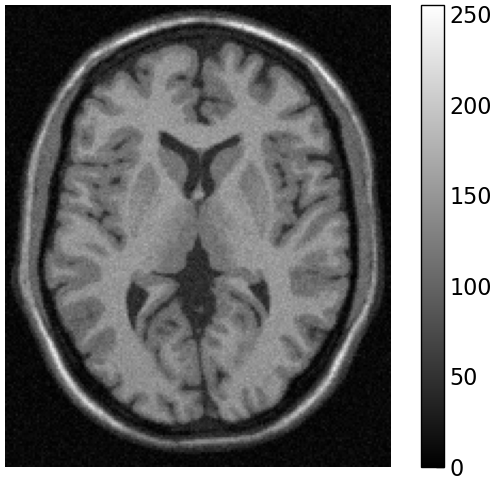
\includegraphics[width=0.21\textwidth]{images/ej_1/ImagenA_HDR.png}\label{fig:imagenA_HDR_ej1}}
  \hfill
  \subfloat[]{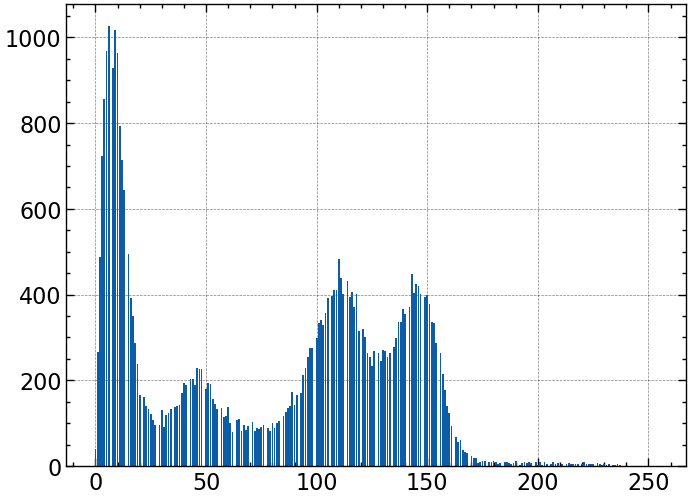
\includegraphics[width=0.27\textwidth]{images/ej_1/hist_HDR.png}\label{fig:hist_HDR_ej1}}
  \hfill
  \caption{imagen original (a) y su histograma (b). Imagen procesada mediante el algoritmo de \textit{contrast streching} (c) y su histograma (d).}
  \label{fig:figuras_ej_1}
\end{figure}

Notar que la escala de grises de la imagen original(Figura \ref{fig:imagenA_ej1}) tiene un valor máximo de $219$, mientras que la imagen procesada (Figura \ref{fig:imagenA_HDR_ej1}) tiene un valor máximo de $255$. Si bien en los histogramas de las figuras \ref{fig:hist_ej1} y \ref{fig:hist_HDR_ej1} no se observa a simple vista una diferencia significativa, la observación anterior corrobora el correcto funcionamiento del algoritmo.


% --------------- EJ 2 ---------------------
\subsection*{Ejercicio 2}
En base a la \texttt{ImagenA.pgm}, inicialmente se llevó a cabo el algoritmo de ecualización del histograma. Este algoritmo busca optimizar el rango dinámico de la imagen, redistribuyendo las intensidades de los píxeles de manera que el histograma resultante sea uniforme. En la Figura \ref{fig:figuras_ej_2} se observa tanto la imagen original como la ecualizada, conjunto con sus respectivos histogramas.

\begin{figure}[htbp]
  \centering
  \subfloat[]{\includegraphics[width=0.21\textwidth]{images/ej_2/ImagenA.png}\label{fig:imagenA_ej2}}
  \hfill
  \subfloat[]{\includegraphics[width=0.27\textwidth]{images/ej_2/hist.png}\label{fig:hist_ej2}}
  \hfill
  \subfloat[]{\includegraphics[width=0.21\textwidth]{images/ej_2/ImagenA_eq.png}\label{fig:imagenA_eq_ej2}}
  \hfill
  \subfloat[]{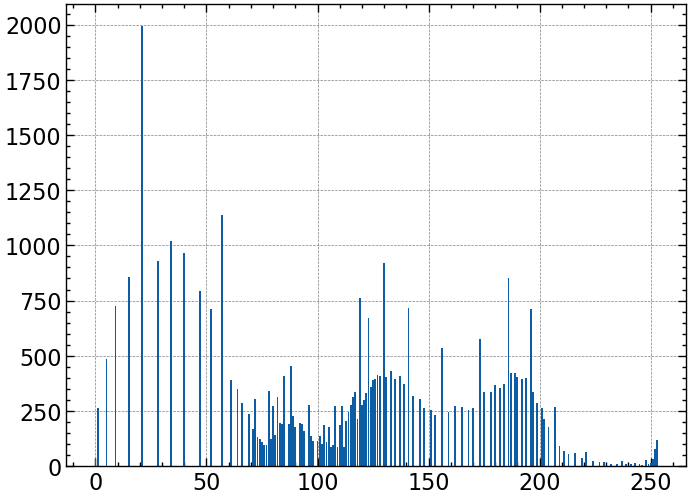
\includegraphics[width=0.27\textwidth]{images/ej_2/hist_eq.png}\label{fig:hist_eq_ej2}}
  \hfill
  \caption{(a) imagen original (b) y su histograma. (c) Imagen ecualizada (d) y su histograma.}
  \label{fig:figuras_ej_2}
\end{figure}

Se puede observar a simple vista que la imagen ecualizada (Figura \ref{fig:imagenA_eq_ej2}) es más brillante que la original (Figura \ref{fig:imagenA_ej2}), en donde la escala de grises indica que la primera alcanza mayores valores de intensidad. En el histograma de la Figura \ref{fig:hist_eq_ej2} se observa que las intensidades de los pixeles se encuentran más redistribuidas respecto al histograma de la Figura \ref{fig:hist_ej2}. Por ejemplo se puede ver que la concentración de los valores de intensidad de los pixeles que se encontraban en el rango de $\approx [0, 50]$ en la imagen original, se encuentran ahora en el rango de $\approx [0, 100]$ en la imagen ecualizada. Esto comprueba el correcto funcionamiento del algoritmo de ecualización.

Diferentes transformaciones $s = T(r)$ pueden ser aplicadas a la imagen, donde s y r denotan la intensidad del pixel de la imagen transformada y original respectivamente. Una de ellas es la \textit{transformación de threshold}, en donde los valores de intensidad que no superen un cierto umbral son mapeados a $0$, y los que lo superen son mapeados a $25$5. En la Figura \ref{fig:figuras_ej_2_threshold} se observa la imagen procesada mediante el algoritmo de \textit{threshold}, con un umbral de $128$.

\begin{figure}[htbp]
  \centering
  \subfloat[]{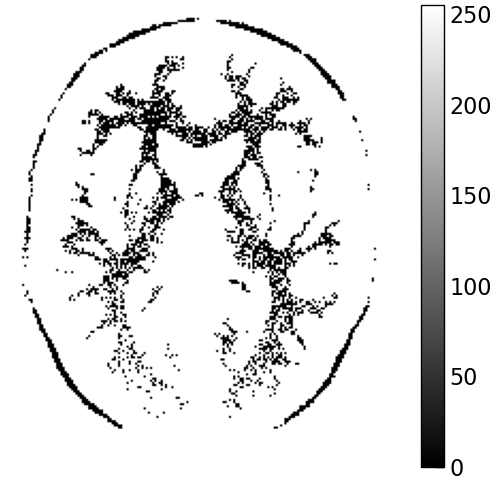
\includegraphics[width=0.21\textwidth]{images/ej_2/ImagenA_threshold.png}\label{fig:imagenA_threshold_ej2}}
  \hfill
  \subfloat[]{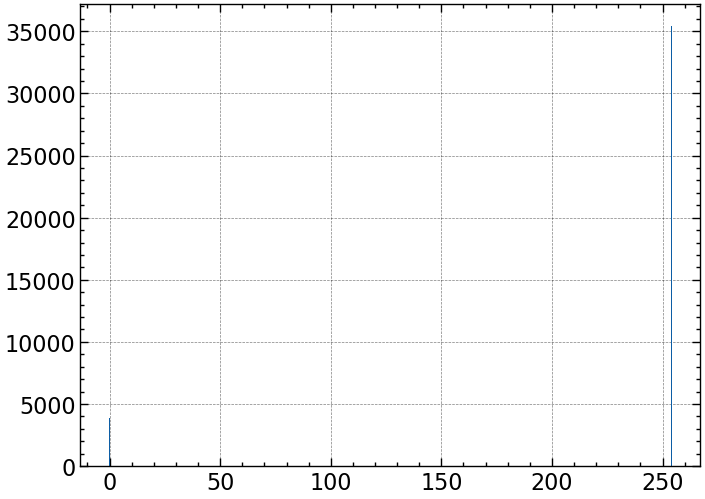
\includegraphics[width=0.27\textwidth]{images/ej_2/hist_threshold.png}\label{fig:hist_threshold_ej2}}
  \hfill
  \caption{(a)imagen con una transformación de threshold con umbral de $128$ (b) y su histograma.}
  \label{fig:figuras_ej_2_threshold}
\end{figure}

Este algoritmo es útil para segmentar la imagen en dos regiones, ya sea para visualizar alguna zona de interés o para utilizar de máscara en otro algoritmo, entre otros. En la Figura \ref{fig:hist_threshold_ej2} se observa que la imagen procesada tiene un histograma con dos picos, uno en $0$ y otro en $255$. Esto confirma el correcto funcionamiento del algoritmo de \textit{threshold}.

Otro tipo de transformación que se puede aplicar a la imagen es la \textit{transformación gamma}. Se define mediante la ecuación $s = c \cdot r^{\gamma}$, donde $c$ es una constante para ajustar los valores de las intensidades y $\gamma$ es el parámetro de la transformación(para que los valores de salida esten entre $0$ y $255$, $c = 255/$max\{imagen\}). Notar que para $\gamma < 1$ se ``dilatan'' las intensidades, en cambio para $\gamma > 1$ se ``contraen''. En la Figura \ref{fig:figuras_ej_2_gamma} se observan la imágenes en las cuales e aplicó la \textit{transformación gamma}, para distintos $\gamma$.

\begin{figure}[H]
  \centering
  \subfloat[]{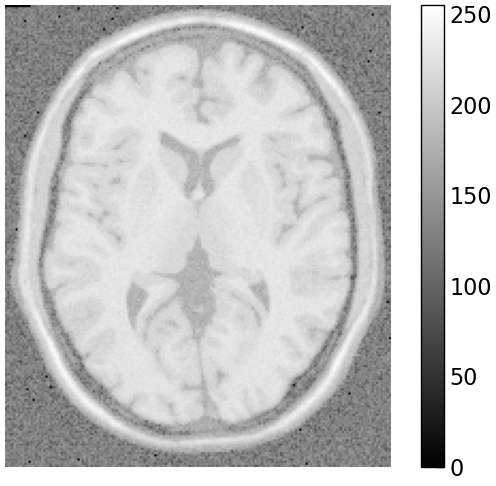
\includegraphics[width=0.21\textwidth]{images/ej_2/ImagenA_gamma_0_2.png}\label{fig:imagenA_gamma_0.2}}
  \hfill
  \subfloat[]{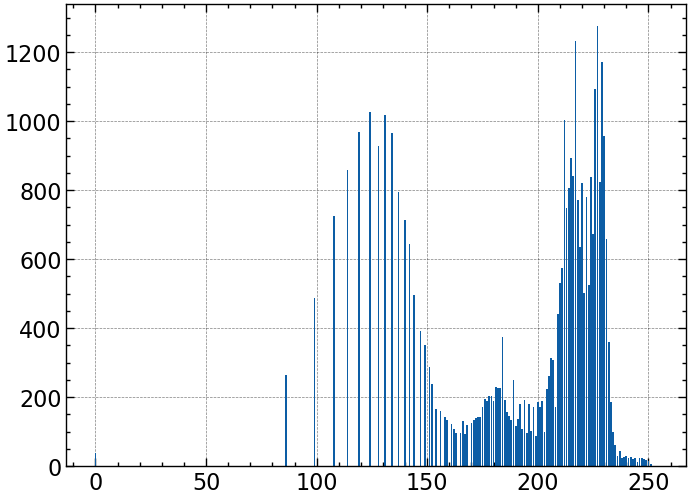
\includegraphics[width=0.27\textwidth]{images/ej_2/hist_gamma_0_2.png}\label{fig:hist_gamma_0.2}}
  \hfill
  \subfloat[]{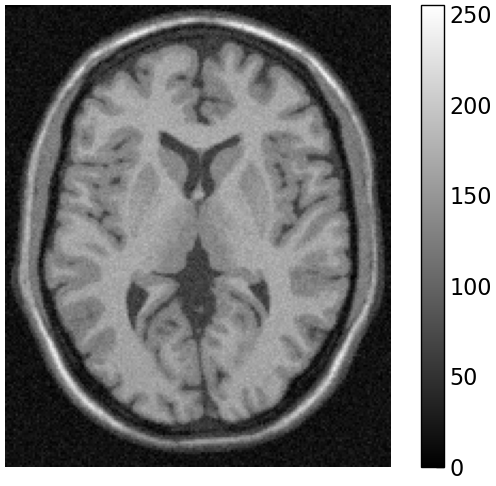
\includegraphics[width=0.21\textwidth]{images/ej_2/ImagenA_gamma_0_8.png}\label{fig:imagenA_gamma_0.8}}
  \hfill
  \subfloat[]{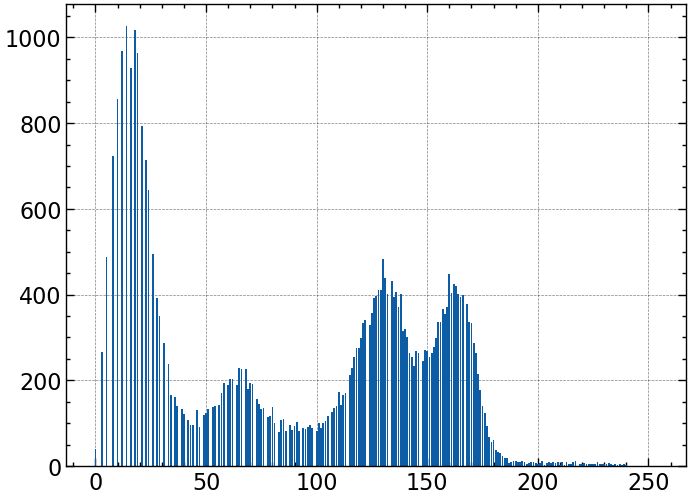
\includegraphics[width=0.27\textwidth]{images/ej_2/hist_gamma_0_8.png}\label{fig:hist_gamma_0.8}}
  \hfill
  \subfloat[]{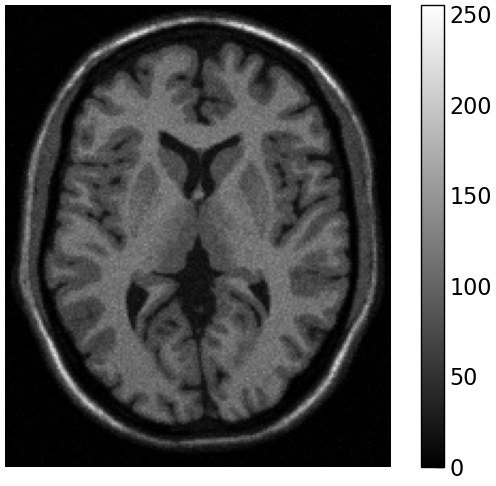
\includegraphics[width=0.21\textwidth]{images/ej_2/ImagenA_gamma_1_5.png}\label{fig:imagenA_gamma_1.5}}
  \hfill
  \subfloat[]{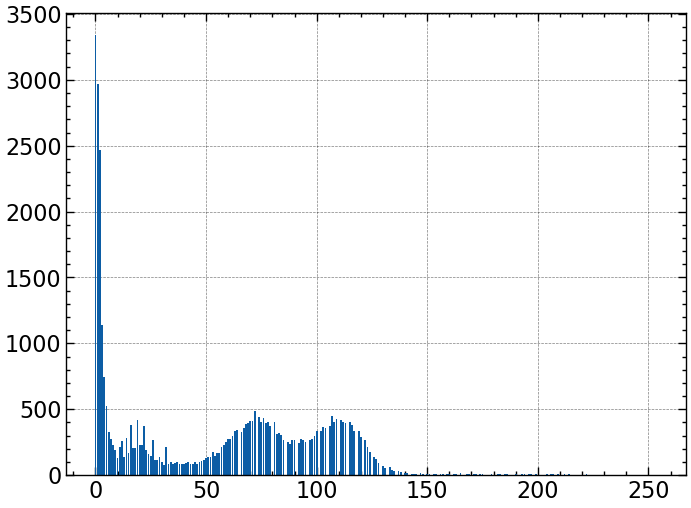
\includegraphics[width=0.27\textwidth]{images/ej_2/hist_gamma_1_5.png}\label{fig:hist_gamma_1.5}}
  \hfill
  \subfloat[]{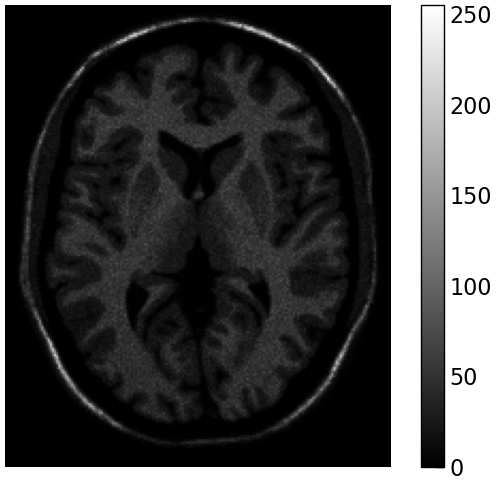
\includegraphics[width=0.21\textwidth]{images/ej_2/ImagenA_gamma_3.png}\label{fig:imagenA_gamma_3}}
  \hfill
  \subfloat[]{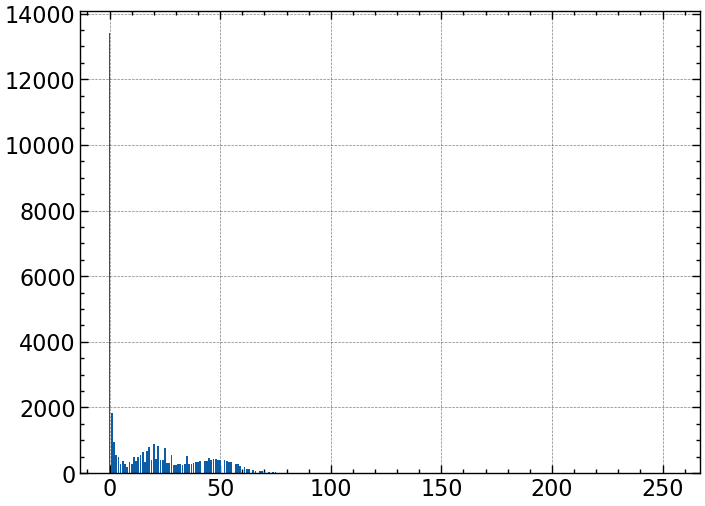
\includegraphics[width=0.27\textwidth]{images/ej_2/hist_gamma_3.png}\label{fig:hist_gamma_3}}
  \hfill
  \caption{imagen procesada mediante una \textit{transformación gamma} conjunto con sus histogramas para diferentes valores de $\gamma$: (a-b) $\gamma = 0.2$, (c-d) $\gamma = 0.8$, (e-f) $\gamma = 1.5$, (g-h) $\gamma = 3$.}
  \label{fig:figuras_ej_2_gamma}
\end{figure}

En la Figura \ref{fig:figuras_ej_2_gamma} se observa que para $\gamma = 0.2$ (Figura \ref{fig:imagenA_gamma_0.2}) la imagen se encuentra más brillante que la original, mientras que a medida que se incrementa el valor de $\gamma$ hasta $\gamma = 3$ (ver figuras \ref{fig:imagenA_gamma_0.8}, \ref{fig:imagenA_gamma_1.5} y \ref{fig:imagenA_gamma_3}) las imagenes se tornan más oscura. Los histogramas de las figuras \ref{fig:hist_gamma_0.2}, \ref{fig:hist_gamma_0.8}, \ref{fig:hist_gamma_1.5} y \ref{fig:hist_gamma_3} confirman esta observación debida a la dilatación y contracción de las intensidades de los pixeles, discutidas en el párrafo anterior.

Finalmente, se realizó la diferencia entre la imagen original y las imagenes procesadas mediante el algoritmo de \textit{threshold} y la \textit{transformación gamma} (se elijió $\gamma = 0.2$ y $3$). En la Figura \ref{fig:figuras_ej_2_diff} se observan las imagenes resultantes.

\begin{figure}[htbp]
  \centering
  \subfloat[]{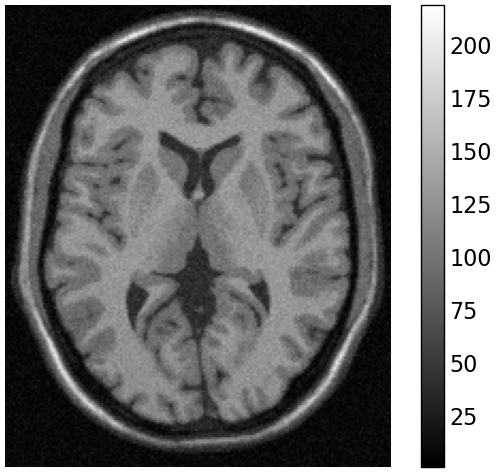
\includegraphics[width=0.21\textwidth]{images/ej_2/ImagenA_diff_thr.png}\label{fig:imagenA_diff_thr}}
  \hfill
  \subfloat[]{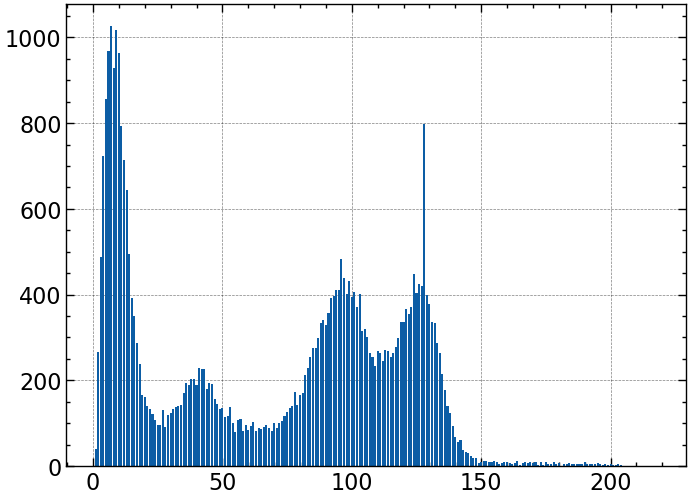
\includegraphics[width=0.27\textwidth]{images/ej_2/hist_diff_thr.png}\label{fig:hist_diff_thr}}
  \hfill
  \subfloat[]{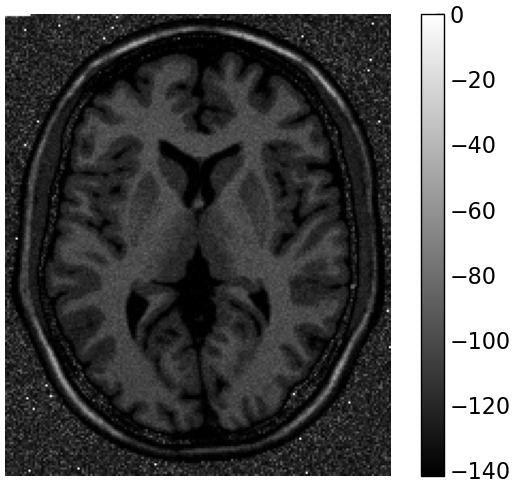
\includegraphics[width=0.21\textwidth]{images/ej_2/ImagenA_diff_gamma_0_2.png}\label{fig:imagenA_diff_gamma_0.2}}
  \hfill
  \subfloat[]{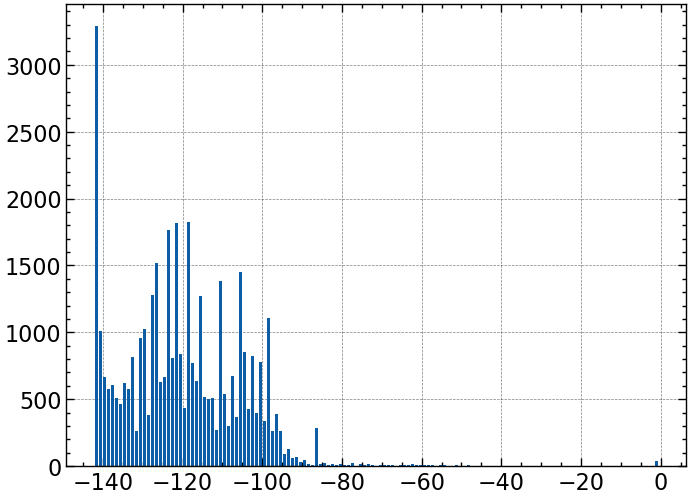
\includegraphics[width=0.27\textwidth]{images/ej_2/hist_diff_gamma_0_2.png}\label{fig:hist_diff_gamma_0.2}}
  \hfill
  \subfloat[]{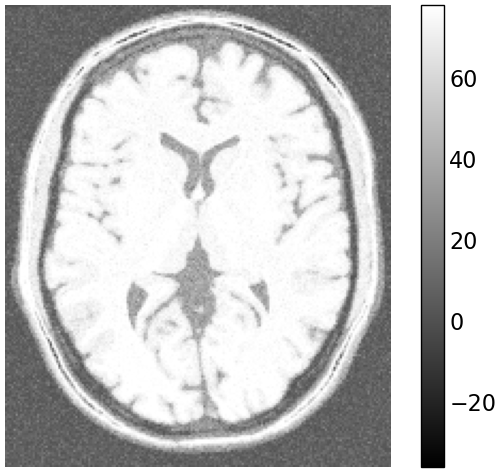
\includegraphics[width=0.21\textwidth]{images/ej_2/ImagenA_diff_gamma_3.png}\label{fig:imagenA_diff_gamma_3}}
  \hfill
  \subfloat[]{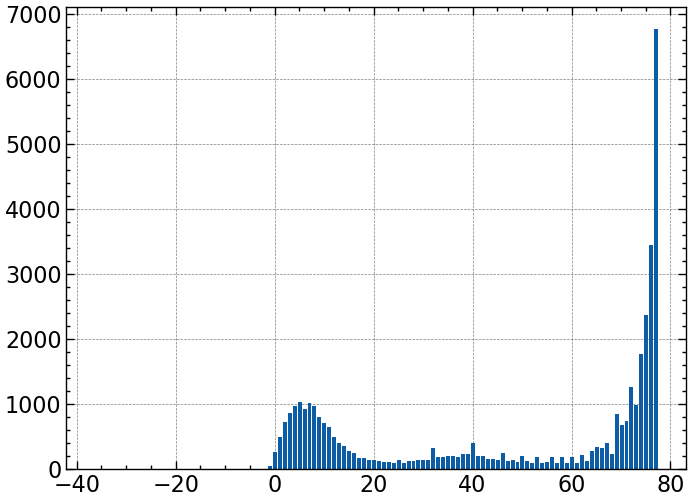
\includegraphics[width=0.27\textwidth]{images/ej_2/hist_diff_gamma_3.png}\label{fig:hist_gamma_diff_3}}
  \hfill
  \caption{imágenes y sus respectivos histogramas de la diferencia entre la imagen original y la imagen transformada mediante las siguientes operaciones: (a-b) transformación de \textit{threshold}, (c-d) transformación \textit{gamma} con un parámetro $\gamma = 0.2$, y (e-f) transformación \textit{gamma} con un parámetro $\gamma = 3$.}
  \label{fig:figuras_ej_2_diff}
\end{figure}

En la Figura \ref{fig:imagenA_diff_thr}, se aprecia que la imagen resultante presenta un histograma (ver Figura \ref{fig:hist_diff_thr}) en el cual se han eliminado las intensidades superiores a $128$ debido al umbral de la transformación de \textit{threshold}. En la Figura \ref{fig:imagenA_diff_gamma_0.2}, la imagen resulta más opaca, y su histograma (ver Figura \ref{fig:hist_diff_gamma_0.2}) muestra que las intensidades superiores se agruparon en valores inferiores. Por otro lado, la imagen de la Figura \ref{fig:imagenA_diff_gamma_3} es más brillante, y su histograma (ver Figura \ref{fig:hist_gamma_diff_3}) indica que las intensidades inferiores se agruparon en valores superiores. Este último efecto se debe a que la transformación \textit{gamma} con $\gamma = 0.2$ dilata las intensidades hacia valores mayores, mientras que la transformación \textit{gamma} con $\gamma = 3$ contrae las intensidades hacia valores inferiores. En consecuencia, al realizar la diferencia, la primera muestra intensidades más bajas, y la segunda, intensidades más altas. Cabe aclarar que los valores negativos se deben a que se presentan los resultados crudos de la diferencia, sin aplicar el mapeo de intensidades a valores entre $0$ y $255$.

% --------------- EJ 3 ---------------------
\subsection*{Ejercicio 3}
Se exploraron diferentes algoritmos de interpolación para la \texttt{ImagenC.pgm}, para llevarla desde su tamaño original $128 \times 128$ hasta un tamaño de $1024 \times 1024$. Inicialmente, se implementó el algoritmo de interpolación del vecino más cercano. Este algoritmo consiste en asignar a cada píxel de la imagen nueva el valor del píxel más cercano de la imagen original. Luego, se implementó el algoritmo de interpolación bilineal, en el cual la intensidad resultante es una combinación lineal de los valores de los píxeles vecinos de la imagen original. Finalmente, se implementó el algoritmo de interpolación bicúbica mediante la función \href{https://docs.opencv.org/3.4/da/d54/group__imgproc__transform.html#ga47a974309e9102f5f08231edc7e7529d}{\texttt{cv2.resize}} del modulo \texttt{openCV} en \texttt{Python}. 

\begin{figure}[htbp]
  \centering
  \subfloat[]{\includegraphics[width=0.24\textwidth]{images/ej_3/ImagenC.png}\label{fig:imagenC_ej_3}}
  \hfill
  \subfloat[]{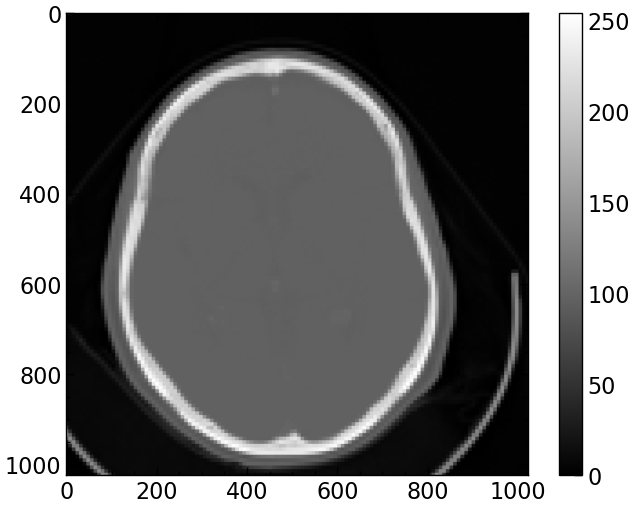
\includegraphics[width=0.24\textwidth]{images/ej_3/ImagenC_resize_narest.png}\label{fig:imagenC_resize_narest}}
  \hfill
  \subfloat[]{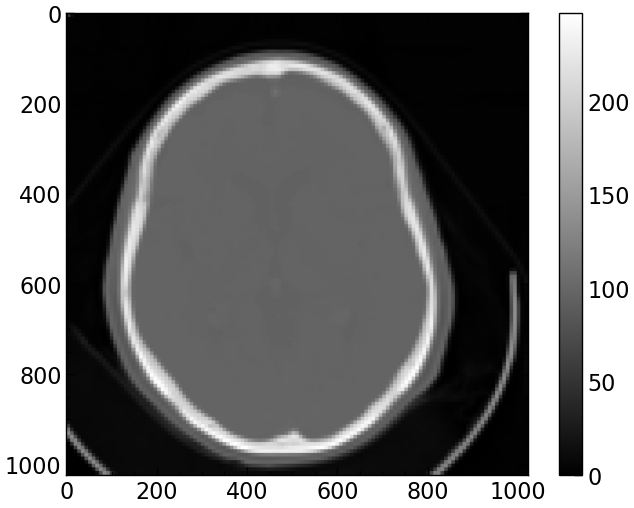
\includegraphics[width=0.24\textwidth]{images/ej_3/ImagenC_resize_bilineal.png}\label{fig:imagenC_resize_bilineal}}
  \hfill
  \subfloat[]{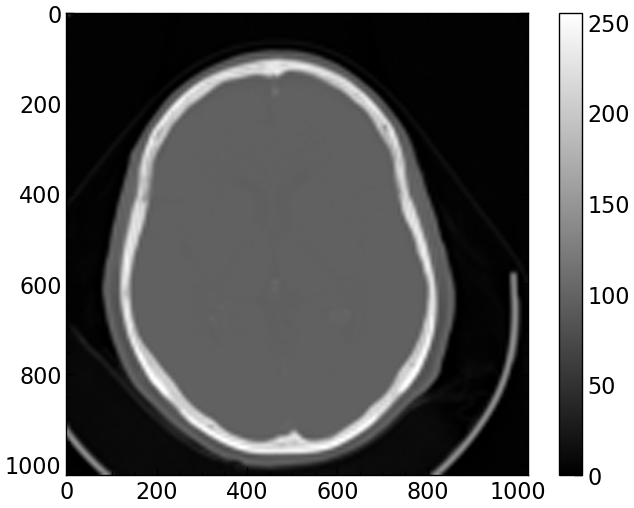
\includegraphics[width=0.24\textwidth]{images/ej_3/ImagenC_resize_bicubic.png}\label{fig:imagenC_resize_bicubic}}
  \hfill
  \caption{(a) imagen original de $124 \times 124$. Imagenes con tamaño de $1024 \times 1024$ procesadas mediante los algoritmos de interpolación: (b) vecino más cercano, (c) bilineal y (d) bicúbica.}
  \label{fig:figuras_ej_3}
\end{figure}

En la Figura \ref{fig:figuras_ej_3} se observa que la imagen resultante de la interpolación del vecino más cercano (Figura \ref{fig:imagenC_resize_narest}) presenta una gran cantidad de artefactos, como el efecto de ``pixelado'', el cual agranda el tamaño de los pixeles, especialmente en los bordes. Por otro lado, en la imagen resultante de la interpolación bilineal (Figura \ref{fig:imagenC_resize_bilineal}) se reducen estos efectos, pero se sigue observando un efecto de pixeleado en los bordes. Finalmente, la imagen resultante de la interpolación bicúbica (Figura \ref{fig:imagenC_resize_bicubic}) presenta la menor cantidad de artefactos y un mayor efecto de suavizado en los bordes, disminuyendo el pixeleado.
% La Figura \ref{fig:figuras_ej_3} revela que la imagen después de la interpolación del vecino más cercano (\ref{fig:imagenC_resize_narest}) muestra notables artefactos, incluyendo un efecto de "pixelado" que agranda los píxeles, especialmente en los bordes. La interpolación bilineal (\ref{fig:imagenC_resize_bilineal}) reduce estos efectos, pero aún se observa el pixelado en los bordes. La interpolación bicúbica (\ref{fig:imagenC_resize_bicubic}) presenta la menor cantidad de artefactos y un suavizado superior en los bordes.

% --------------- EJ 4 ---------------------
\subsection*{Ejercicio 4}

Se implementan filtros pasabajos para las imágenes \texttt{ImagenA.pgm} e \texttt{ImagenC.pgm}. Se utilizaron diferentes kernels para el filtro con el objetivo de comparar los resultados. Para la implementación de un filtro pasabajos, el kernel que se utiliza es una matriz de la forma $\overline{\overline{k} }  = \frac{1}{n^2} \overline{\overline{\mathbb{I}}}_{n\times n}$, donde $\overline{\overline{\mathbb{I}}}_{n\times n}$ es la matriz identidad de tamaño $n \times n$. Para el proceso de filtrado se realiza la convolución discreta de la imagen con el kernel, en donde el valor de cada píxel de la imagen resultante es el promedio de los valores de los píxeles vecinos de la imagen original. Las Figuras \ref{fig:figuras_ej_4_A} y \ref{fig:figuras_ej_4_C} muestran los resultados para kernels de tamaño $3 \times 3$, $5 \times 5$, y $7 \times 7$ en las imágenes \texttt{ImagenA.pgm} y \texttt{ImagenC.pgm}, respectivamente. Cada imagen se procesó utilizando el método "same" para mantener el tamaño de la imagen original.



\begin{figure}[htpb]
  \centering
  \subfloat[]{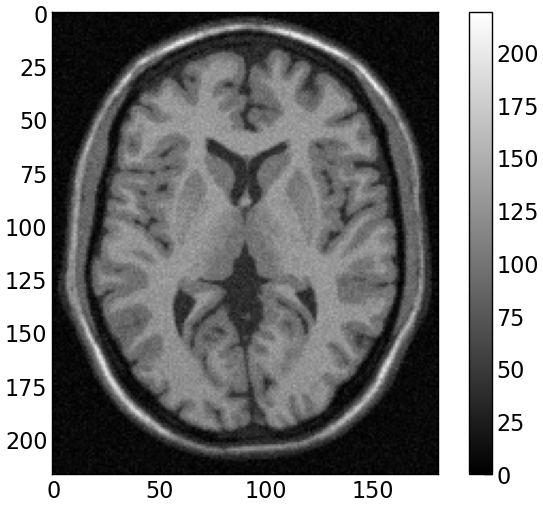
\includegraphics[width=0.24\textwidth]{images/ej_4/ImagenA.png}\label{fig:imagenA_ej_4}}
  \hfill
  \subfloat[]{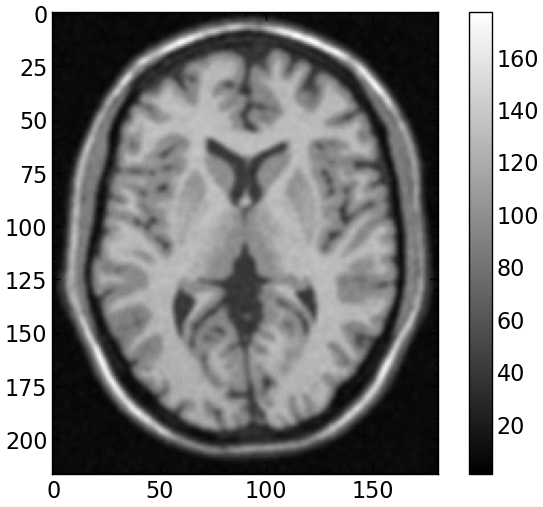
\includegraphics[width=0.24\textwidth]{images/ej_4/ImagenA_3x3.png}\label{fig:imagenA_3x3}}
  \hfill
  \subfloat[]{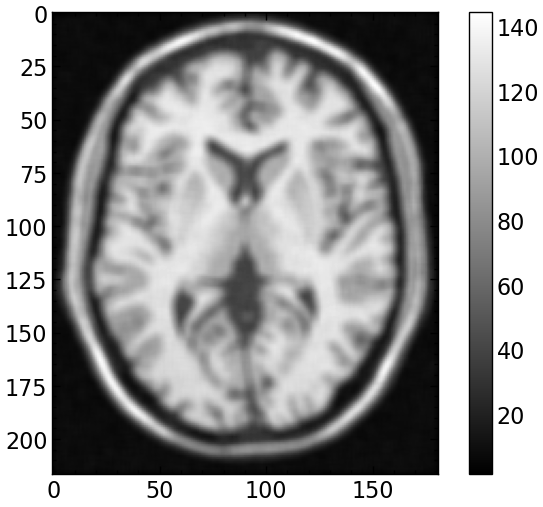
\includegraphics[width=0.24\textwidth]{images/ej_4/ImagenA_5x5.png}\label{fig:imagenA_5x5}}
  \hfill
  \subfloat[]{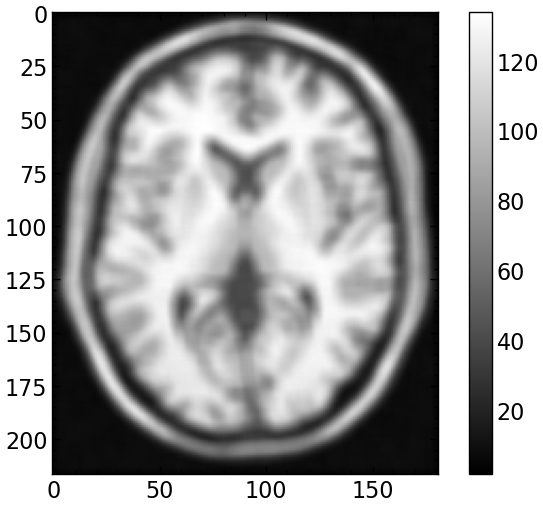
\includegraphics[width=0.24\textwidth]{images/ej_4/ImagenA_7x7.png}\label{fig:imagenA_7x7}}
  \hfill
  \caption{(a) Imagen original \texttt{ImagenA}. Imágenes resultantes después de aplicar un filtro pasabajos con kernels de tamaño (b) $3 \times 3$, (c) $5 \times 5$, y (d) $7 \times 7$.}
  \label{fig:figuras_ej_4_A}
\end{figure}

\begin{figure}[htpb]
  \centering
  \subfloat[]{\includegraphics[width=0.24\textwidth]{images/ej_4/ImagenC.png}\label{fig:imagenC_ej_4}}
  \hfill
  \subfloat[]{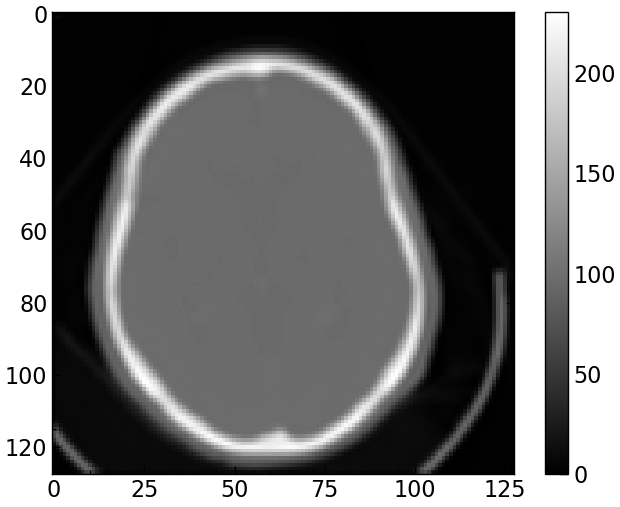
\includegraphics[width=0.24\textwidth]{images/ej_4/ImagenC_3x3.png}\label{fig:imagenC_3x3}}
  \hfill
  \subfloat[]{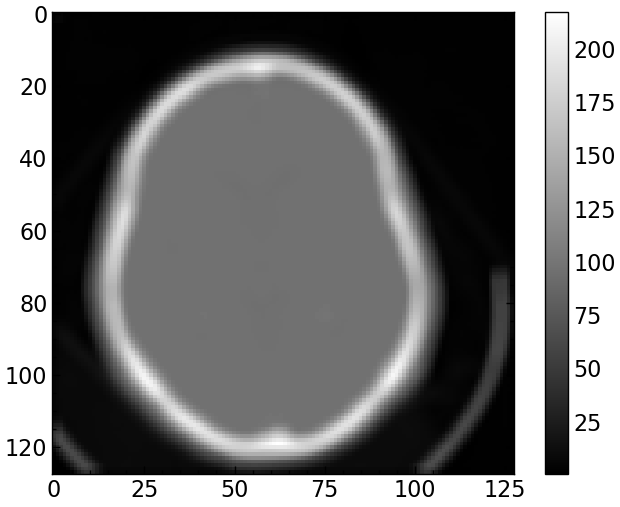
\includegraphics[width=0.24\textwidth]{images/ej_4/ImagenC_5x5.png}\label{fig:imagenC_5x5}}
  \hfill
  \subfloat[]{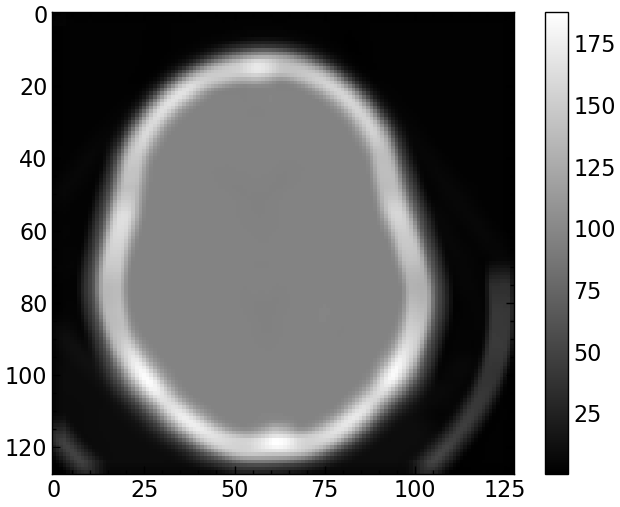
\includegraphics[width=0.24\textwidth]{images/ej_4/ImagenC_7x7.png}\label{fig:imagenC_7x7}}
  \hfill
  \caption{(a) Imagen original \texttt{ImagenC}. Imágenes resultantes después de aplicar un filtro pasabajos con kernels de tamaño (b) $3 \times 3$, (c) $5 \times 5$, y (d) $7 \times 7$.}
  \label{fig:figuras_ej_4_C}
\end{figure}

Tanto en las diferentes imágenes de la Figura \ref{fig:figuras_ej_4_A} como en las de la Figura \ref{fig:figuras_ej_4_C}, se observa que a medida que se incrementa el tamaño del kernel, la imagen resultante se encuentra más suavizada. Si bien el efecto de suavizado reduce el ruido y pixeleado de la imagen, también disminuye la nitidez de los bordes. Por ello es importante elegir un tamaño de kernel adecuado para el filtro, dependiendo de la imagen y el efecto deseado. Además, se visualiza que el metodo de filtrado ``same'' mantiene el tamaño de la imagen original. La ventaja frente al método ``valid'' es que se evita la perdida de información de los bordes de la imagen, que se hace más notorio para kernels de mayor dimensión.

% --------------- EJ 5 ---------------------
\subsection*{Ejercicio 5}
Se exploró la transformada rápida de Fourier para implementar filtros en el dominio de la frecuencia, con el objetivo de eliminar ruido que presenta cierta periodicidad en la imagen. 

Para ello, se realizó la transformada de Fourier de la imagen \texttt{superman.pgm} y se graficó el modulo de la transformada, como se muestra en la Figura \ref{fig:superman_fft}. En ella se puede observar que la transformada de Fourier de la imagen presenta picos de intensidad en ciertas zonas, lo que podría indicar presencia de artefactos.

\begin{figure}[htbp]
  \centering
  \subfloat[]{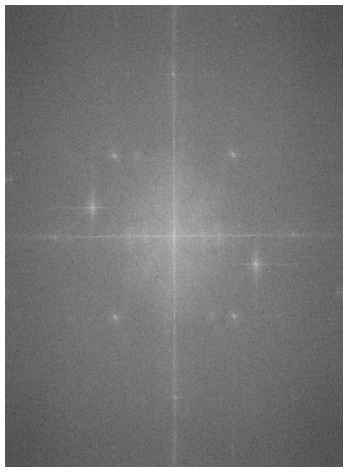
\includegraphics[width=0.24\textwidth]{images/ej_5/superman_fft.png}\label{fig:superman_fft}}
  \hfill
  \subfloat[]{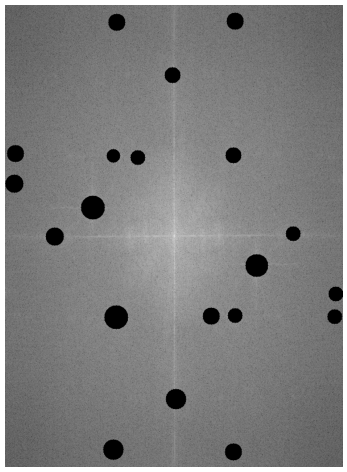
\includegraphics[width=0.24\textwidth]{images/ej_5/circulos.png}\label{fig:circulos}}
  \hfill
  \caption{(a) modulo de la transformada de Fourier de la imagen \texttt{superman}. (b) máscara aplicada sobre la transformada para filtrar el ruido.}
  \label{fig:figuras_fft_ej_5}
\end{figure}

Para eliminar estos artefactos observados en la Figura \ref{fig:superman_fft}, se aplicó una máscara en forma de círculos trazados manualmente, como se muestra en la Figura \ref{fig:circulos}, en cada lugar donde se encontraban estos picos de intensidades. Luego, se estableció el valor de los píxeles de la máscara en $0$, para que al realizar la transformada inversa de Fourier, se elimine el ruido de la imagen. En la Figura \ref{fig:figuras_fft_filtrada_ej_5} se observa la imagen original y la imagen filtrada.

\begin{figure}[htbp]
  \centering
  \subfloat[]{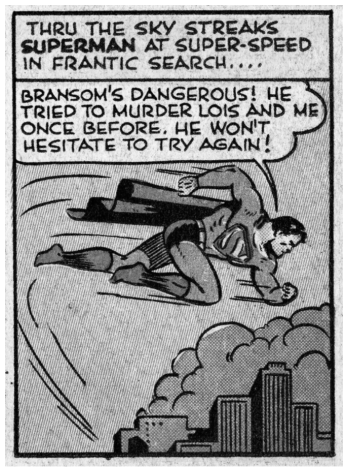
\includegraphics[width=0.24\textwidth]{images/ej_5/superman.png}\label{fig:superman}}
  \hfill
  \subfloat[]{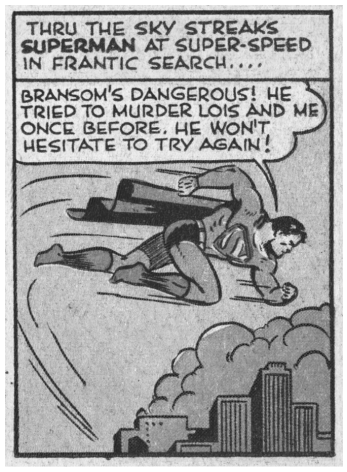
\includegraphics[width=0.24\textwidth]{images/ej_5/superman_filtered.png}\label{fig:superman_fft_filtrada}}
  \hfill
  \caption{(a) imagen original \texttt{superman}. (b) imagen filtrada mediante la transformada de Fourier.}
  \label{fig:figuras_fft_filtrada_ej_5} 
\end{figure}

En la Figura \ref{fig:superman} se visualiza una componente periódica en la textura de la imagen, producto del proceso de impresión de la imagen. Luego de la aplicación del filtro anteriormente mencionado, gran parte de esta componente periódica se elimina, como se observa en la Figura \ref{fig:superman_fft_filtrada}. 

% --------------- EJ 6 ---------------------
\subsection*{Ejercicio 6}
Se introdujo ruido gaussiano a la imagen \texttt{ImagenA.pgm} con el propósito de evaluar los filtros \textit{Unsharp} y \textit{Highboost}. La generación del ruido gaussiano se realizó mediante la función \href{https://numpy.org/doc/stable/reference/random/generated/numpy.random.normal.html}{\texttt{numpy.random.normal}} en \texttt{Python}, con una media de $0$ y una desviación estándar de $1$. A los valores obtenidos se les multiplicó por una constante denominada "level", que cuantifica el nivel de ruido agregado. La Figura \ref{fig:figuras_ej_6} presenta tanto la imagen original como la imagen con ruido gaussiano.

\begin{figure}[htbp]
  \centering
  \subfloat[]{\includegraphics[width=0.24\textwidth]{images/ej_6/ImagenA.png}\label{fig:imagenA_ej_6}}
  \hfill
  \subfloat[]{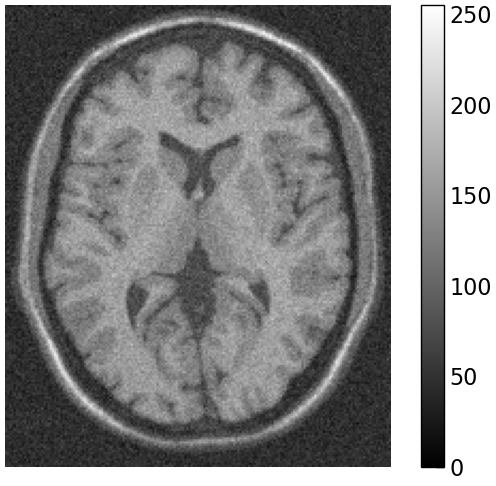
\includegraphics[width=0.24\textwidth]{images/ej_6/ImagenA_noisy.png}\label{fig:imagenA_gauss}}
  \hfill
  \caption{(a) Imagen original \texttt{ImagenA}. (b) Imagen con ruido gaussiano con nivel = $10$.}
  \label{fig:figuras_ej_6}
\end{figure}

La imagen afectada por el ruido, como se muestra en la Figura \ref{fig:imagenA_gauss}, se utilizó para evaluar el desempeño de los filtros pasaaltos. En este contexto, $f(x, y)$ denota la imagen original a filtrar y $g(x, y)$ la imagen filtrada mediante un filtro pasabajos. La expresión para un filtro pasa altos se define mediante $f_{\text{filtrada}}(x, y) = A f(x, y) - g(x, y)$, donde $A$ representa un factor de ponderación o peso. En el caso $A=1$, corresponde al filtro \textit{Unsharp}; para otros valores de $A$, se refiere al filtro \textit{Highboost}. La Figura \ref{fig:figuras_ej_6_filtered} muestra el resultado de aplicar estos filtros con distintos valores de $A$.

\begin{figure}[htbp]
  \centering
  \subfloat[]{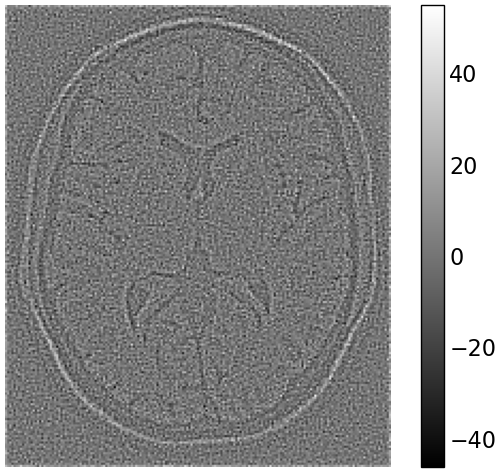
\includegraphics[width=0.24\textwidth]{images/ej_6/ImagenA_unsharp.png}\label{fig:imagenA_unsharp}}
  \hfill
  \subfloat[]{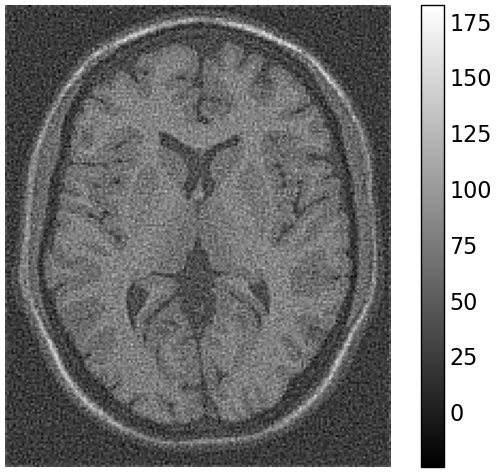
\includegraphics[width=0.24\textwidth]{images/ej_6/ImagenA_highboost_1_5.png}\label{fig:imagenA_highboost_1_5}}
  \hfill
  \subfloat[]{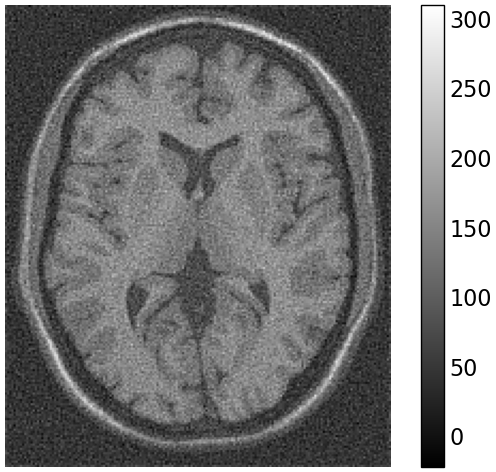
\includegraphics[width=0.24\textwidth]{images/ej_6/ImagenA_highboost_2.png}\label{fig:imagenA_highboost_2}}
  \hfill
  \subfloat[]{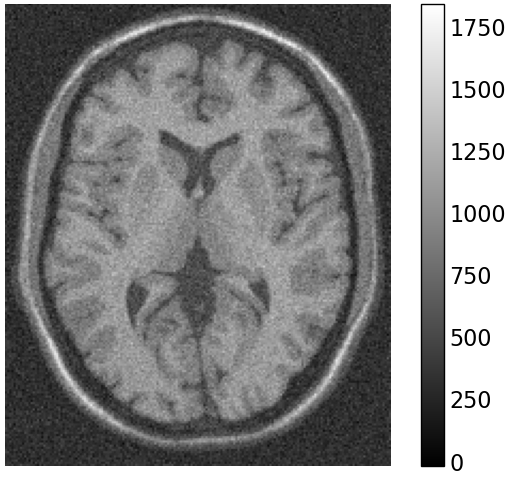
\includegraphics[width=0.24\textwidth]{images/ej_6/ImagenA_highboost_8.png}\label{fig:imagenA_highboost_8}}
  \hfill
  \caption{(a) Imagen filtrada con filtro unsharp. Imágenes filtradas con el filtro highboost con parámetro $A$: (b) $A = 1.5$, (c) $A = 2$, y (d) $A = 8$.}
  \label{fig:figuras_ej_6_filtered}
\end{figure}

Para evaluar la performance del filtro para diferente valores del parámetro $A$, se define una métrica la suma de todos los elementos del valor absoluto de la diferencia termino a termino, es decir $d = \sum \left|a_{ij} - b_{ij}\right|$, donde $a_{ij}$ y $b_{ij}$ corresponden al elemento $i, j$ de la matriz de la imagen filtrada y la original respectivamente. Notar que a menor distancia $d$, mayor es la performance del filtro ya que difiere menos de la imagen original. En la Figura \ref{fig:distance} se muestra la distancia obtenida para diferentes valores del parámetro $A$.

\begin{figure} [htbp]
  \centering
  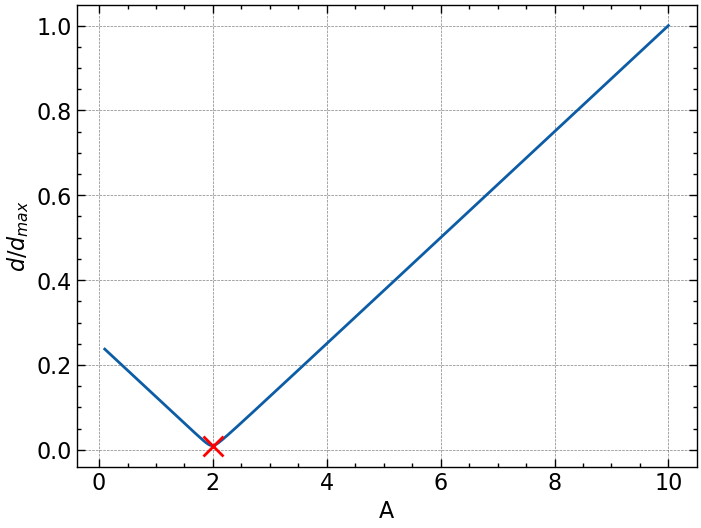
\includegraphics[width=0.5\textwidth]{images/ej_6/distance.png}
  \caption{resultados obtenidos de la metrica resultante para diferentes valores del parámetro $A$ del filtro highboost.}
  \label{fig:distance}
\end{figure}

En la gráfica de la Figura \ref{fig:distance} se puede observar que la distancia se minimiza para $A = 2$. El crecimiento lineal para $A > 2$ se puede explicar debido a la forma en que se calcula el filtro \textit{highboost}. A medida que se incrementa el valor de $A$, la imagen $g(x, y)$ (filtrada con pasabajos) es menos significativa ya que el peso de la imagen $f(x, y)$ original crece proporcionalmente. Por lo tanto, es de esperar que la diferencia aumente proporcional con el parametro. Un argumento similar explica porque decrece linealmente hasta el mínimo, pero en lugar de pesar más la imagen original, tiene mayor peso la imagen filtrada con pasabajos.

% --------------- EJ 7 ---------------------
\subsection*{Ejercicio 7}

Se utilizaron imágenes adquiridas con el CT HiSpeed con el objetivo de medir la relación señal ruido (\textit{SNR} por sus siglas en inglés) y el ancho de la \textit{point spread function} (\textit{PSF}) (definido por el FWHM). 

Inicialmente se midió la \textit{SNR}, definida mediante $SNR = \mu / \sigma$, donde $\mu$ es el valor medio de la imagen y $\sigma$ es la desviación estándar. Para ello, se seleccionó una región de interés \textit{ROI} en donde se quiere medir el valor medio y el desvío estándar de la imagen. En la Figura \ref{fig:figuras_ej_7} se observa la imagen original y la imagen con la \textit{ROI} marcada.

\begin{figure}[htbp]
  \centering
  \subfloat[]{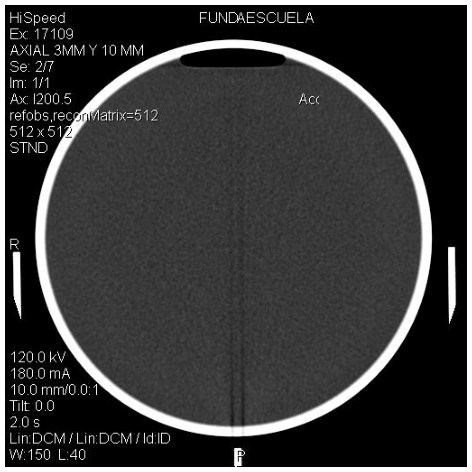
\includegraphics[width=0.24\textwidth]{images/ej_7/AAA0002.png}\label{fig:AAA0002}}
  \hfill
  \subfloat[]{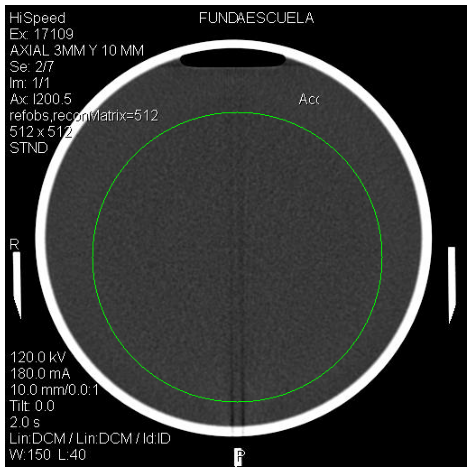
\includegraphics[width=0.24\textwidth]{images/ej_7/AA0002_circle.png}\label{fig:AA0002_ROI}}
  \hfill
  \caption{(a) imagen original adquirida con el CT HiSpeed (\texttt{AAA0002.pgm}). (b) imagen con la región de interés seleccionada.}
  \label{fig:figuras_ej_7}
\end{figure}

Se mantuvo la misma \textit{ROI} para cada todos los cortes (2, 3 y 4) dado que se trataba de la misma imagen, pero obtenida con diferentes valores de corriente eléctrica. En la Figura \ref{fig:SNR_vs_I} se graficó la relación señal ruido en función de la corriente utilizada para adquirir la imagen.

\begin{figure} [htbp]
  \centering
  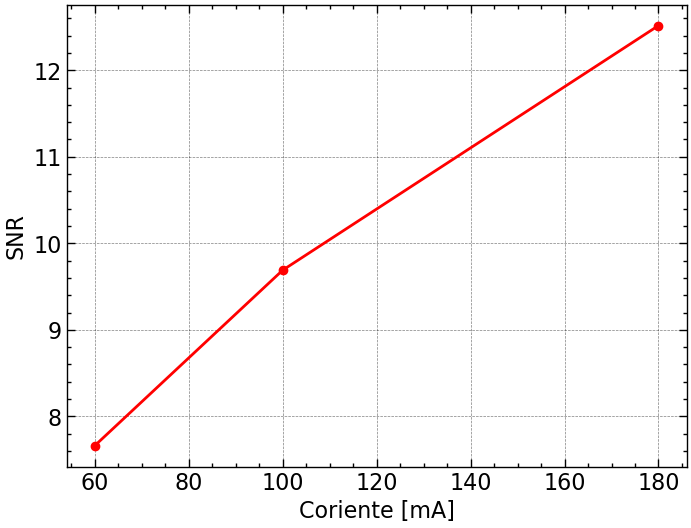
\includegraphics[width=0.5\textwidth]{images/ej_7/SNR_corriente.png}
  \caption{SNR en función de la corriente utilizada para adquirir la imagen de CT HiSpeed.}
  \label{fig:SNR_vs_I}
\end{figure}

En la Figura \ref{fig:SNR_vs_I} se observa que la SNR aumenta a medida que se incrementa la corriente utilizada para adquirir la imagen. Esto se debe a que a mayor corriente, mayor es la cantidad de fotones que llegan al detector, lo que disminuye el ruido de la imagen.

Por último, se midió la \textit{PSF} sobre el punto definido por los cortes $11$ al $14$. En la Figura \ref{fig:figuras_ej_7_b} se observa la imagen original y la linea transversal sobre la cual se midió la \textit{PSF}. Esta linea se mantuvo para cada uno de los cortes analizados. 

\begin{figure}[htbp]
  \centering
  \subfloat[]{\includegraphics[width=0.24\textwidth]{images/ej_7/AAA0011.png}\label{fig:AAA0011}}
  \hfill
  \subfloat[]{\includegraphics[width=0.24\textwidth]{images/ej_7/AAA0011_corte.png}\label{fig:AA00011_corte}}
  \hfill
  \caption{(a) imagen original capturada con el CT HiSpeed (\texttt{AAA0011.pgm}). (b) Imagen ampliada con una línea roja que delimita la región seleccionada para medir la PSF.}
  \label{fig:figuras_ej_7_b}
\end{figure}

Se obtuvieron los valores de los pixeles delimitados por la línea roja que se muestra en la Figura \ref{fig:AA00011_corte} para medir la \textit{PSF} sobre el punto blanco del centro. Para ello, primero se identifica el máximo de la señal, dado que se quiere medir la $PSF$ de un punto blanco, y se buscan los valores de los pixeles más cercanos que se encuentran a la mitad de la altura del máximo, o el más cercano estrictamente menor (el hecho de elegir el menor es una cuestión de criterio). En la Figura \ref{fig:PSF} se muestra, a modo de ejemplo, la señal resultante y los valores necesarios para el FWHM del corte 11. Los demás cortes se midieron de la misma manera y la forma de la grafica es similar, pero con diferentes artefactos.

\begin{figure}[htbp]
  \centering
  \includegraphics[width=0.45\textwidth]{images/ej_7/PSF.png}
  \caption{Señal resultante y valores necesarios para el FWHM del corte 11. La línea punteada verde representa la mitad del máximo de la señal, y las dos cruces verdes indican los valores de los pixeles más cercanos al máximo, que se encuentran a la mitad de la altura del máximo.}
  \label{fig:PSF}
\end{figure}

La linea punteada verde de la Figura \ref{fig:PSF} indica la mitad del máximo de la señal, y las dos cruces verdes indican los valores de los pixeles más cercanos al máximo, que se encuentran a la mitad de la altura del máximo. El PSF se calcula mediante la resta de los valores de estos pixeles. Los valores obtenidos para los diferentes cortes se muestran en la Tabla \ref{tab:PSF}.

\begin{table}[H]
  \centering
  \begin{tabular}{|c|c|}
  \hline
  \textbf{Corte} & \textbf{PSF [px]} \\ \hline
  11             & 6           \\ \hline
  12             & 15           \\ \hline
  13             & 7           \\ \hline
  14             & 5           \\ \hline
  \end{tabular}
  \caption{Valores de PSF obtenidos para los diferentes cortes analizados.}
  \label{tab:PSF}
\end{table}

En la Tabla \ref{tab:PSF} se observa que el valor de la \textit{PSF} es mayor para el corte 12, lo que indica que la resolución espacial es menor en este corte. En esta imagen se observó una especie de anillo concentrico al punto blanco, lo que indica fenómenos de interferencia, produciendo artefactos que afectan la resolución espacial.


% ------------------ CONCLUSION ---------------------
\section{Conclusiones}

En conclusión, se implementaron diversos algoritmos de procesamiento de imágenes, destacando su aplicabilidad en diferentes contextos. La transformación de \textit{threshold} resultó útil para la segmentación de imágenes, mientras que la transformación \textit{gamma} proporcionó un medio versátil para ajustar el contraste, permitiendo dilatar ($\gamma < 1$) o contraer($\gamma > 1$) el histograma. Además, se verificó que el método de ecualización tiende a generar histogramas más uniformes, lo que permite utilizar todo el rango dinámico de la imagen.

Se implementaron diferentes algoritmos de interpolaciones para aumentar el tamaño de la imágen. Como resultado, el método de vecino más cercano tiende a generar artefactos, como agrandar el tamaño de los pixeles. La interpolación bilineal redujo estos efectos, pero la interpolación bicúbica presentó la menor cantidad de artefactos y un mayor efecto de suavizado en los bordes, disminuyendo el pixeleado. Sin embargo, es importante tener en cuenta que la interpolación bicúbica es más costosa computacionalmente que la interpolación bilineal.


Para el caso del filtrado se constató que los filtros pasa bajos son útiles para reducir el ruido, aunque con la desventaja de afectar la nitidez de los bordes. La aplicación de la transformada de Fourier resultó eficaz en la eliminación de artefactos periódicos. En cuanto a los filtros pasa altos, se estableció que el parámetro óptimo (que presenta una métrica menor) para el filtro \textit{highboost} es $A = 2$.

Por último, se midió que la \textit{SNR} adquiridas en el CT HiSpeed aumenta a medida que se incrementa la corriente utilizada para adquirir la imagen, lo cual es esperable dado a que se incrementa la cantidad de fotones que llegan al detector, disminuyendo el ruido de la imagen. Además, se observó que el valor de la \textit{PSF} es mayor para el corte 12, debido a los efectos de interferencia, resultando en una menor resolución espacial.

\end{document}
